\subsection{Evaluierung}
Damit die Ausarbeitung beginnen kann, muss eine gute Kombination für die zukünftigen Hardware-Komponenten zusammengestellt werden. Diese Kombination sollte auf den Spezifikationen basieren, die vom Projektbetreuer Simon Köldorfer definiert wurden. Diese Spezifikationen umfassen die grundsätzliche Verwendung eines Displays, die IP66-Tauglichkeit des Gehäuses, die Witterungstauglichkeit der Anzeige sowie die Möglichkeit, die Anzeigeseite zu ändern, wobei nicht spezifiziert ist, wie dies umgesetzt werden soll. Die Spannungsversorgung muss außerdem als 24VAC/DC ausgeführt sein. Schließlich sollte die Lösung auch wirtschaftlich sinnvoll sein, falls sich entschieden wird, diese Anzeige fortan an mehreren oder sogar allen Lüftungsgeräten anzubringen. Die genaueren Spezifikationen befinden sich im Kapitel \ref{aufgabenstellung}.\\
Trotz dieser Definitionen blieb genug Freiheit, um mehrere Möglichkeiten zusammenzustellen und somit dem nachzugehen, was für diese Diplomarbeit am passendsten ist. 
Folgend werden alle vier Varianten gelistet, die später auch so innerhalb eines Meetings dem Projektbetreuer näher gebracht wurden. Anzumerken ist, dass die angegebenen Preise möglicherweise zur Realität etwas abweichen können.
\paragraph{Variante A}
Die erste Variante beinhaltet als einzige den Mikrocontroller Arduino. Genauer gesagt handelt es sich um den Arduino Mega. Hier war die Grundidee, ein kleines 3.5 Zoll Display mit 1-2 Buttons herzustellen und alles in einer IP66 tauglichen, kleinen Box zu verstauen. 
Die positiven Aspekte dieser Variante beziehen sich sowohl auf den Preis als auch auf die Verfügbarkeit der Teile. Variante A hat mit Abstand den niedrigsten Gesamtpreis, dieser liegt bei ungefähr 63,00 € und die Verfügbarkeit ist stets gegeben. Auch in Bezug auf die Haltbarkeit ist es ein Plus-Punkt, da Witterungen dem Gehäuse nichts ausmachen, und im Falle, dass es doch kaputtgehen würde, es leicht und günstig zu ersetzen ist. Die Schwierigkeit der Umsetzung ist ebenso auf einem akzeptablen Level; problematisch könnte es hier mit der Weiterleitung oder der Terminierung der Modbus-Signale werden. Schwierigkeiten existieren aber auch bei der Benutzerfreundlichkeit, da die Bedienung mit 2 Buttons komplizierter bzw. umfangreicher wäre als mit einem. Die Dokumentationen für die Libraries sind auch eher kurz gehalten, wie beispielsweise bei der Library \enquote{ModbusMaster}.
\begin{figure}[ht]
	\centering
	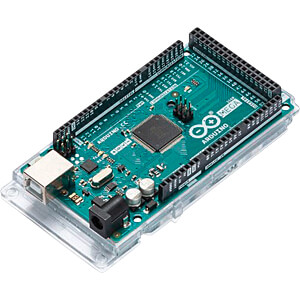
\includegraphics[width=0.5\linewidth]{Bilder/ARDUINO_MEGA.jpg}
	\caption{Arduino Mega (Quelle: \url{https://cdn-reichelt.de/bilder/web/artikel_ws/A300/ARDUINO_MEGA_01_NEU.jpg})}
	\label{fig:arduino_mega}
\end{figure}
\paragraph{Variante B}
\paragraph{Variante C}
\paragraph{Variante D}